%---------------------------------------------------------------------------------------------------
%		docker.tex
%
%	This file contains the sections that describe the Docker project and its architecture
% models
%
%	Author: Andrea Meneghinello
% Version: 0.1
%	Table of changes:
%		12/03/2016 -> document definition
%---------------------------------------------------------------------------------------------------
\section{Docker containers}
\label{sec:problemSpace-docker}
Docker started its life as an open-source project at “dotCloud”, a cloud-centric PaaS company, in early
2013.

Initially Docker was the natural extension of the technology that company had developed to run its cloud
business on thousands of servers. It was written in Go, a statically typed programmed language developed
by Google with syntax loosely based on C. In the next months the company, having regard to the obtained
results, joined the Linux Foundation and changed its name to Docker Inc. and announced that was shifting
its focus on the development of Docker and its ecosystem.

Docker is an open platform for developing, shipping and running applications, it is designed to deliver
software as faster as possible thanks to a shorter cycle between writing and running code. It allows the
separation of the application from the infrastructure and treats the last one like a managed application.
It allows this combining a lightweight container virtualization platform with workflows and tools
that help in managing and deploying applications.

In its core, Docker provides a way to run almost any application securely isolated in a container.
Isolation and security allow to run many containers simultaneously on the same host. Its lightweight
nature, which run without the extra load of a hypervisor, means that we can get more out from the
hardware.

Tools and a platform surround containers so they can help in several tasks:

\begin{itemize}
	\item{getting applications (and supporting components) into containers;}
	\item{distributing and shipping containers to different teams for further development and testing;}
	\item{deploying applications to production environment, whether it is in local data-centre or in the
		cloud.}
\end{itemize}

In the following sections we will discuss about its architecture, and how it is able to manage users'
data and resolve the dependency-hell problem. Finally we will do brief a digression about the state-of-art
in security.

\subsection{Docker architecture}
\label{sec:problemSpace-docker-architecture}
Docker is based on a client-server architecture: the \keyword{client} and \keyword{daemon}. Docker
client ``talks'' with the daemon, which does the hardest work of building, running and distributing
the containers. Users cannot directly interact with the daemon: they must write commands for it 
through the client.

Both the Docker client and the daemon can run on the same system, or it is possible to connect the
first one to a remote daemon. They can communicate via sockets or through a RESTful \acs{api}.

The Docker ecosystem, shown in Figure \ref{img:problemSpace-docker-architecture-architecture}, is
composed by the following components: \keyword{images}, \keyword{registries} and finally
\keyword{containers}.

\begin{figure}
	\centering{}
	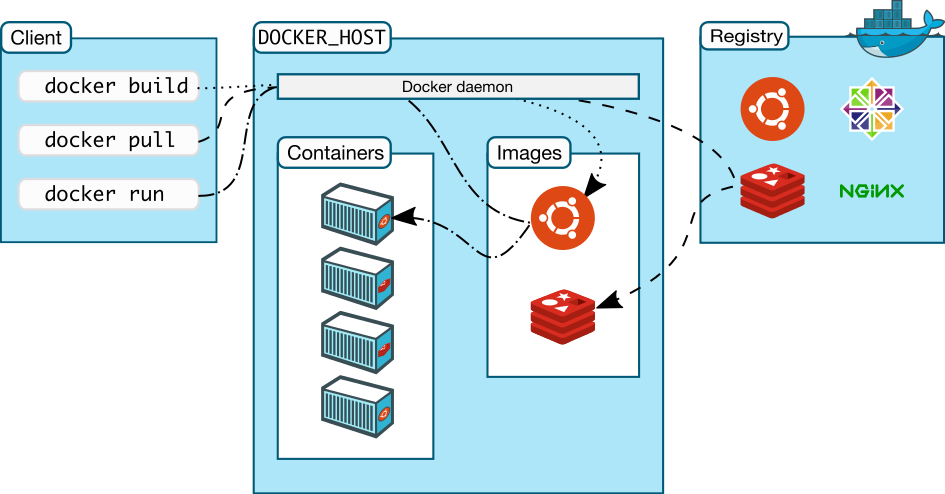
\includegraphics[width=0.8\textwidth]{chapters/problem/images/docker-architecture.png}
	\caption[Docker architecture overview]{Docker architecture overview. We can see that a command
		received by the Docker client is forwarded to the Docker daemon which manages the container
		life-cycle. To the right there is the registry that holds the published images.}
	\label{img:problemSpace-docker-architecture-architecture}
\end{figure}

A Docker image is a read-only template that Docker uses to create the runnable container; it provides
a simple way to build new images or to update existing ones. A Docker image is created defining a
file (called dockerfile), that contains a description of the application/service (and its dependencies)
that will be contained when it runs. Each image consists of a series of layers; they are combined together
into a single and compact image thanks to the use of \ac{ufs}\footnote{We will discuss about \ac{ufs}
afterwards when we will cover how data are managed.}. Docker images are the build component of the
Docker ecosystem.

Docker registries hold images; these can be public or private stores from which we can upload or
download images. The most famous public registry is provided by Docker and it is called Docker Hub, while
private ones are created and maintained by private companies for proprietary use. Registries serve a
huge collection of existing ready-to-use images. They are the distribution component of the Docker
ecosystem.

Finally Docker containers are an isolated and secure application platform, similar to a system directory
that holds everything that is needed by the application to run. When users decide to deploy a new
container, they make a request to the Docker client; the client forwards the request to the Docker
daemon, which reads the corresponding image and uses it to “give life” to the container. Docker containers
can be run, started, stopped, moved, and deleted easily. They are the run component of the Docker ecosystem.

With Docker containers we can achieve isolation and resource control (important features of SaaS)
through the use of namespaces and cgroups (see Section \ref{sec:problemSpace-virtualization-types})

To manage isolation and resource control, Docker largely uses Linux-kernel features, but different kernels
can have contrasting interfaces for the same functionalities. This is the reason why Docker, since v0.9,
replaced the old \ac{lxc} execution environment (which contains cgroups and namespaces) with
\keyword{LibContainer} (shown in Figure \ref{img:problemSpace-docker-architecture-libcontainer}).

\begin{figure}
	\centering{}
	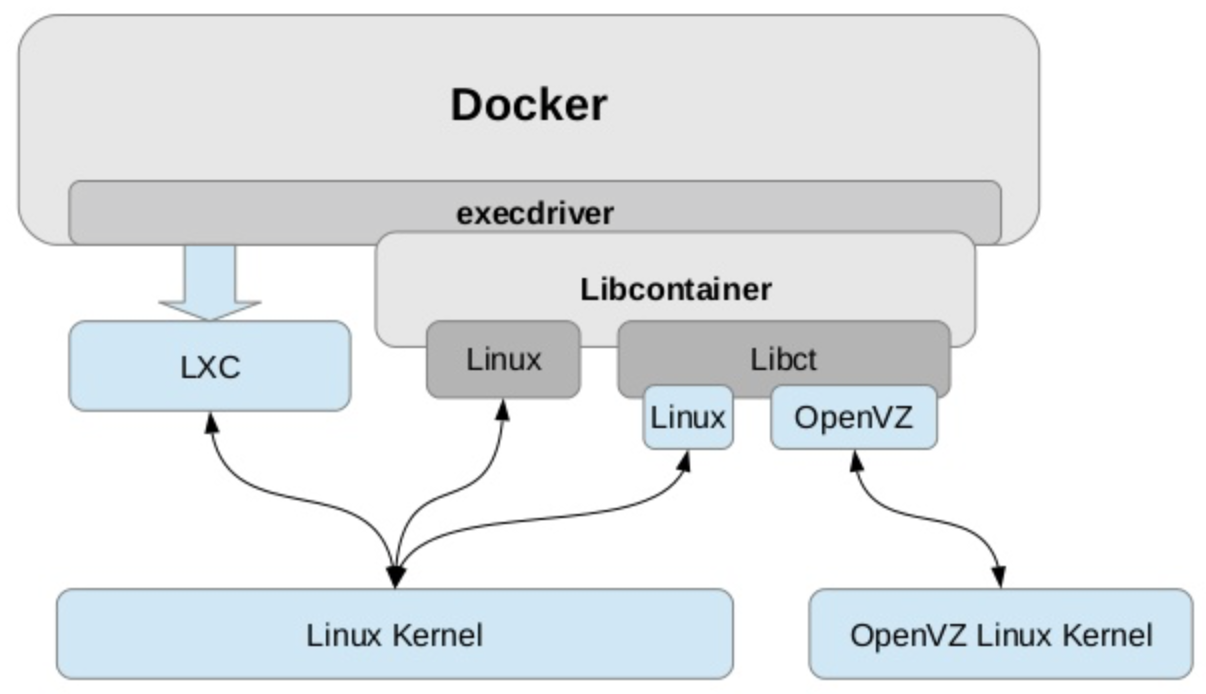
\includegraphics[width=0.6\textwidth]{chapters/problem/images/libcontainer.png}
	\caption[Docker libcontainer overview]{Now Docker execution environment is separated from the underlying
		\acs{os} though the introduction of LibContainers.}
	\label{img:problemSpace-docker-architecture-libcontainer}
\end{figure}

LibContainer is now the default Docker execution environment. It is meant to be a cross-system abstraction
layer being an attempt to standardize the way applications are packed up, delivered and run in isolation.
Thus, container features available in Linux kernel \acs{api} are provided as a unique library in a
consistent way; it addresses the problem of having an unique kernel \acs{api} and several implementations.

LibContainer has become a stand alone project, after Docker decided to donate it to the open-source community,
therefore other developers (Google, Parallels, RedHat, Ubuntu and others) can contribute to improve its development.

As we just stated, Docker containers are executed in isolation, but this do not prevent them to share data using
the network. Containers can be connected together in two different ways: through a connection based on 
IP-address/TCP-port or the link feature.

In the first case containers, that have an unique IP address, must open outward a TCP port on which they can
listen for incoming connections. Even if it seems reasonable using this type of network connection to share
data, this can instead lead to security problems because connections can arrive also from the web. On the other
hand establishing a connection, between containers, through the link feature is like building a \ac{vpn};
which means less risks for the safety factor, because the connection is only available between different
containers behind the same firewall\footnote{We will analyse in Chapter REF the benefit of this feature.}.

\subsection{Data management}
\label{sec:problemSpace-docker-dataManagement}
Docker images are read-only templates from which Docker containers are lunched. Each image consists of
a series of layers combined into a single image using the \acf{ufs} technology.

One reason why Docker is lightweight derives from these layers. When a developer changes a Docker image,
e.g. to deploy a new version of an application, a new layer is built. Thus, rather than replacing
or entirely rebuilding the whole image, as in case of \ac{vm}s, only that layer is added or updated thus
making the Docker image distribution faster and simpler; just this one will be distributed.

\ac{ufs} (shown in Figure 6) is a stackable \ac{fs} which implements the union-mount features. That allows
to specify a series of different \ac{fs} (called branches) which are finally presented as a virtual
and coherent one, even though the branches come from different \ac{fs}. This process is commonly
referred to as namespaces unification.

\begin{figure}
	\centering{}
	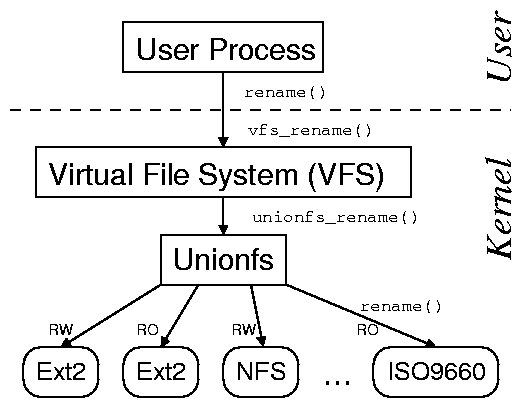
\includegraphics[width=0.4\textwidth]{chapters/problem/images/unionfs.png}
	\caption[Docker \ac{ufs} overview]{Example of file renaming using the \acf{ufs}. The user's process
		see only one logical file and it is responsibility of \acf{vfs} to correctly map the rename command
		to different underlying \acf{fs}.}
	\label{img:problemSpace-docker-architecture-unionfs}
\end{figure}

\ac{ufs} uses a simple priority model which gives a unique priority to each branch . If a file exists
in multiple branches, only the copy in higher priority branch will be shown. It also allows some branches
to be read-only, but as long as at least one of them is readable and writeable, \ac{ufs} uses ``copy-on-write''
semantic to provide an illusion that all branches are writeable.

To maintain \ac{fs} integrity, Docker containers are composed by read-only layers except for the 
upper one. Another key characteristic of the Docker containers is that its \ac{fs} is designed to
be ephemeral. Then if a container contains a service that write files or data when it is running 
(like a database service), all of them will be lost after container termination. Thus in a future
launch of the same, into it we can only find the work environment (configured as described in 
the dockerfile) but without the previously generated files or data.

To ensure that this situation does not happens, there is the need to separate the container from
data life-cycle. Ideally we want that the generated data is not destroyed or tied to the container
life-cycle and can thus be reused. To achieve this, Docker provides the concepts of \keyword{data-volumes}
and \keyword{data-volumes container}.

A data-volume is a specially designed directory in the container that is able to “bypass” the \ac{ufs}.
It is initialized when the container is created and, by default, it is not deleted when the container
is stopped or when there is no container that reference it. Data-volumes are independently updated,
shareable across different containers and mountable in read-only mode too. This key feature is provided
through a symbolic link (also known as soft-link) that points to a \ac{fs} location in the \acs{os}
underlying docker daemon. Hence data will persist after container termination, and in a future launch
of it the only necessary thing to retrieve them is to fix the link (through a mount operation made at
container launch time) which point at the correct location in the underlying file-system.

Instead, a data-volume container becomes useful when we want to share data between different containers
or we want to use data from non-persistent containers. They are particular containers that aim to collect
different data-volumes and make them available for other containers.

These two features are useful when we plan to provide a backup, restore or migration features in our
applications.

\subsection{Dependency hell problem}
\label{sec:problemSpace-docker-dependencyHell}
\citeauthor{michaeljang2006} in \cite{michaeljang2006} defines the colloquial term “dependency hell” 
to point out a set of problems. It refers to the frustration problem that software developers deal with
when installing applications with dependencies on specific versions of other software packages. Modern
applications often are assembled from existing components and delegate many tasks to third parties services
and applications, so this problem must not be under-estimated.

The problem may occur in several forms: a huge number of dependencies should be downloaded and locally saved
(large amount of downloading time and storage space may be necessary), long chain of dependencies, conflicting 
dependencies, circular dependencies and finally package manager dependencies (problem encountered when 
the packet manager is not able to download linked dependencies automatically).

Docker allows to fix, implicitly, the cited problems by packaging each component and its dependencies
into a container. In particular, with Docker the following issues cannot be risen:

\begin{itemize}
	\item{\keyword{conflicting dependencies}: we can run different software versions, that require
		different dependencies or many version of them, in various containers. Each one with
		the correct one dependencies;}
	\item{\keyword{missing dependencies}: no dependency can be missing because every one is packaged
		along with the application container;}
	\item{\keyword{platform differencies}: moving from one provider to another is no longer a
		problem if both systems run the Docker daemon; the same container will execute without other
		issues.}
\end{itemize}

\subsection{Security issues}
\label{sec:problemSpace-docker-security}
Docker is becoming an interesting technology in cloud computing world and for this reason we need also
to analyse its intrinsic security issues. Speaking about Docker security, we need to focus on the following
areas: intrinsic security of Linux kernel and its support for namespaces and cgroups features, the weaknesses
of the Docker daemon itself and finally poorly configured images.

Since Docker features lie on Linux kernel, these provide an initial inherent safety. Kernel namespace
feature is the one that provides the first and straightforward form of isolation. Its main purpose is
to grant that processes inside a container cannot be seen or affected, by processes running
in other containers or in the host system. In addition each container gets its own network stack, meaning
that it cannot get a privileged access to the sockets or network interfaces of others. This means that
containers are just like physical machines connected to a common Ethernet switch, because all containers, on
a given Docker host, are placed over bridges interfaces. Cgroups are the key component of the Linux kernel
that provide resource accounting and limiting. They allow security ensuring that each container gets its fair
share of resources (memory, CPU, Disk I/O), and finally preventing a container to bring the system down due to
exhausting of computing resources. So while they do not play a role in preventing one container from accessing or
affecting data of other processes or containers, they are essential to fend off some \ac{dos} attacks, becoming
thus an interesting feature in multi-tenant environments. Both namespaces and cgroups features are available
together since Linux kernel 2.6.26 (released 8 years ago); they have been scrutinized on a large number of
production systems, so their design and their consequent implementations are pretty mature.

Running containers with Docker implies executing the Docker daemon on the host, and currently it requires
root privileges to perform its tasks. Hence only trusted system-users should be allowed to control and dialogue
with it. Docker images can request to the daemon to share directories (data-volumes) between a container
and the underlying host file-system. This means that a malicious user can start a container in which its 
``/host'' directory will be mapped to the ``/'' directory of the underlying host \acs{os}. Hence the container
will be able to alter the host file-system without restrictions while it should not have this permission.
This has a strong security implication when a cloud provider plan to provide a public \acs{api} to deploy
containers. It should be more careful than usual with the parameter checking to make sure that a malicious
user cannot pass crafted parameters causing Docker to create arbitrary containers. For this reason the Docker
REST \acs{api} endpoint is changed using, from version 0.5.2, the UNIX socket instead of a TCP bound on
127.0.0.1; This have been done because the latter are prone to \ac{csrf} attacks. Docker daemon can also be
attacked through images loading from disk or from network. This has been focus of improvements in the community,
especially for images coming from not-trusted networks. Hence from Docker 1.3.2 images are now extracted in a
chrooted sub-process on the Linux platform. In conclusion it is expected that the Docker daemon will run with
restricted privileges, delegating well-audited operations to sub-processes, each one with its own very limited
set of privileges to avoid that malicious containers can exploit vulnerabilities. This will be possible with the
future adoption of the recent improvements in Linux namespaces which includes the user-namespace. Moreover, this
will also solve the problem caused by sharing \ac{fs}s between host and guest, since the user namespace
allows users (including the root user) to be mapped to other users in the host system within containers.

Finally, many security lacks come from wrong configuration provided by the users when they define dockerfiles.
In this scenario common mistakes include software from unknown sources or wrong network configuration that
pave the way for malicious users.